% Options for packages loaded elsewhere
\PassOptionsToPackage{unicode}{hyperref}
\PassOptionsToPackage{hyphens}{url}
\PassOptionsToPackage{dvipsnames,svgnames,x11names}{xcolor}
%
\documentclass[
  11pt,
  a4paper,
]{article}

\usepackage{amsmath,amssymb}
\usepackage{setspace}
\usepackage{iftex}
\ifPDFTeX
  \usepackage[T1]{fontenc}
  \usepackage[utf8]{inputenc}
  \usepackage{textcomp} % provide euro and other symbols
\else % if luatex or xetex
  \usepackage{unicode-math}
  \defaultfontfeatures{Scale=MatchLowercase}
  \defaultfontfeatures[\rmfamily]{Ligatures=TeX,Scale=1}
\fi
\usepackage{lmodern}
\ifPDFTeX\else  
    % xetex/luatex font selection
    \setmainfont[]{Palatino Linotype}
\fi
% Use upquote if available, for straight quotes in verbatim environments
\IfFileExists{upquote.sty}{\usepackage{upquote}}{}
\IfFileExists{microtype.sty}{% use microtype if available
  \usepackage[]{microtype}
  \UseMicrotypeSet[protrusion]{basicmath} % disable protrusion for tt fonts
}{}
\makeatletter
\@ifundefined{KOMAClassName}{% if non-KOMA class
  \IfFileExists{parskip.sty}{%
    \usepackage{parskip}
  }{% else
    \setlength{\parindent}{0pt}
    \setlength{\parskip}{6pt plus 2pt minus 1pt}}
}{% if KOMA class
  \KOMAoptions{parskip=half}}
\makeatother
\usepackage{xcolor}
\usepackage[top=2.4cm,bottom=2.4cm,left=2.5cm,right=2.5cm]{geometry}
\setlength{\emergencystretch}{3em} % prevent overfull lines
\setcounter{secnumdepth}{-\maxdimen} % remove section numbering


\providecommand{\tightlist}{%
  \setlength{\itemsep}{0pt}\setlength{\parskip}{0pt}}\usepackage{longtable,booktabs,array}
\usepackage{calc} % for calculating minipage widths
% Correct order of tables after \paragraph or \subparagraph
\usepackage{etoolbox}
\makeatletter
\patchcmd\longtable{\par}{\if@noskipsec\mbox{}\fi\par}{}{}
\makeatother
% Allow footnotes in longtable head/foot
\IfFileExists{footnotehyper.sty}{\usepackage{footnotehyper}}{\usepackage{footnote}}
\makesavenoteenv{longtable}
\usepackage{graphicx}
\makeatletter
\def\maxwidth{\ifdim\Gin@nat@width>\linewidth\linewidth\else\Gin@nat@width\fi}
\def\maxheight{\ifdim\Gin@nat@height>\textheight\textheight\else\Gin@nat@height\fi}
\makeatother
% Scale images if necessary, so that they will not overflow the page
% margins by default, and it is still possible to overwrite the defaults
% using explicit options in \includegraphics[width, height, ...]{}
\setkeys{Gin}{width=\maxwidth,height=\maxheight,keepaspectratio}
% Set default figure placement to htbp
\makeatletter
\def\fps@figure{htbp}
\makeatother

\usepackage{booktabs}
\usepackage{longtable}
\usepackage{array}
\usepackage{multirow}
\usepackage{wrapfig}
\usepackage{float}
\usepackage{colortbl}
\usepackage{pdflscape}
\usepackage{tabu}
\usepackage{threeparttable}
\usepackage{threeparttablex}
\usepackage[normalem]{ulem}
\usepackage{makecell}
\usepackage{xcolor}
\makeatletter
\@ifpackageloaded{tcolorbox}{}{\usepackage[skins,breakable]{tcolorbox}}
\@ifpackageloaded{fontawesome5}{}{\usepackage{fontawesome5}}
\definecolor{quarto-callout-color}{HTML}{909090}
\definecolor{quarto-callout-note-color}{HTML}{0758E5}
\definecolor{quarto-callout-important-color}{HTML}{CC1914}
\definecolor{quarto-callout-warning-color}{HTML}{EB9113}
\definecolor{quarto-callout-tip-color}{HTML}{00A047}
\definecolor{quarto-callout-caution-color}{HTML}{FC5300}
\definecolor{quarto-callout-color-frame}{HTML}{acacac}
\definecolor{quarto-callout-note-color-frame}{HTML}{4582ec}
\definecolor{quarto-callout-important-color-frame}{HTML}{d9534f}
\definecolor{quarto-callout-warning-color-frame}{HTML}{f0ad4e}
\definecolor{quarto-callout-tip-color-frame}{HTML}{02b875}
\definecolor{quarto-callout-caution-color-frame}{HTML}{fd7e14}
\makeatother
\makeatletter
\@ifpackageloaded{caption}{}{\usepackage{caption}}
\AtBeginDocument{%
\ifdefined\contentsname
  \renewcommand*\contentsname{Table of contents}
\else
  \newcommand\contentsname{Table of contents}
\fi
\ifdefined\listfigurename
  \renewcommand*\listfigurename{List of Figures}
\else
  \newcommand\listfigurename{List of Figures}
\fi
\ifdefined\listtablename
  \renewcommand*\listtablename{List of Tables}
\else
  \newcommand\listtablename{List of Tables}
\fi
\ifdefined\figurename
  \renewcommand*\figurename{Figure}
\else
  \newcommand\figurename{Figure}
\fi
\ifdefined\tablename
  \renewcommand*\tablename{Table}
\else
  \newcommand\tablename{Table}
\fi
}
\@ifpackageloaded{float}{}{\usepackage{float}}
\floatstyle{ruled}
\@ifundefined{c@chapter}{\newfloat{codelisting}{h}{lop}}{\newfloat{codelisting}{h}{lop}[chapter]}
\floatname{codelisting}{Listing}
\newcommand*\listoflistings{\listof{codelisting}{List of Listings}}
\makeatother
\makeatletter
\makeatother
\makeatletter
\@ifpackageloaded{caption}{}{\usepackage{caption}}
\@ifpackageloaded{subcaption}{}{\usepackage{subcaption}}
\makeatother
\makeatletter
\@ifpackageloaded{sidenotes}{}{\usepackage{sidenotes}}
\@ifpackageloaded{marginnote}{}{\usepackage{marginnote}}
\makeatother

\ifLuaTeX
  \usepackage{selnolig}  % disable illegal ligatures
\fi
\usepackage{bookmark}

\IfFileExists{xurl.sty}{\usepackage{xurl}}{} % add URL line breaks if available
\urlstyle{same} % disable monospaced font for URLs
\hypersetup{
  pdftitle={Recruiting Veterans and Military Family Members Improves Confidence in Elections},
  pdfauthor={Isaiah; Michael J. Hanmer, PhD},
  pdfkeywords={Election Workers, Poll workers, Veterans, Public
opinion, Election administration},
  colorlinks=true,
  linkcolor={blue},
  filecolor={Maroon},
  citecolor={Blue},
  urlcolor={Blue},
  pdfcreator={LaTeX via pandoc}}

%% CAPTIONS
\usepackage{caption}
\DeclareCaptionStyle{italic}[justification=centering]
 {labelfont={bf},textfont={it},labelsep=colon}
\captionsetup[figure]{style=italic,format=hang,singlelinecheck=true}
\captionsetup[table]{style=italic,format=hang,singlelinecheck=true}

%% FONT
% \usepackage{bera}
% \usepackage[charter]{mathdesign}
% \usepackage[scale=0.9]{sourcecodepro}
% \usepackage[lf,t]{FiraSans}
\usepackage{fontawesome}

%% HEADERS AND FOOTERS
\usepackage{fancyhdr}
\pagestyle{fancy}
\rfoot{\Large\sffamily\raisebox{-0.1cm}{\textbf{\thepage}}}
\makeatletter
\lhead{\textsf{\expandafter{\@title}}}
\makeatother
\rhead{}
\cfoot{}
\setlength{\headheight}{15pt}
\renewcommand{\headrulewidth}{0.4pt}
\renewcommand{\footrulewidth}{0.4pt}
\fancypagestyle{plain}{%
\fancyhf{} % clear all header and footer fields
\fancyfoot[C]{\sffamily\thepage} % except the center
\renewcommand{\headrulewidth}{0pt}
\renewcommand{\footrulewidth}{0pt}}

%% MATHS
\usepackage{bm,amsmath}
\allowdisplaybreaks

%% GRAPHICS
\makeatletter
\def\fps@figure{htbp}
\makeatother
\setcounter{topnumber}{2}
\setcounter{bottomnumber}{2}
\setcounter{totalnumber}{4}
\renewcommand{\topfraction}{0.85}
\renewcommand{\bottomfraction}{0.85}
\renewcommand{\textfraction}{0.15}
\renewcommand{\floatpagefraction}{0.8}

%% SECTION TITLES
\usepackage[compact,sf,bf]{titlesec}
\titleformat*{\section}{\Large\sf\bfseries\color[rgb]{0.7,0,0}}
\titleformat*{\subsection}{\large\sf\bfseries\color[rgb]{0.7,0,0}}
\titleformat*{\subsubsection}{\sf\bfseries\color[rgb]{0.7,0,0}}
\titlespacing{\section}{0pt}{2ex}{.5ex}
\titlespacing{\subsection}{0pt}{1.5ex}{0ex}
\titlespacing{\subsubsection}{0pt}{.5ex}{0ex}


%% BIBLIOGRAPHY.

\makeatletter
\@ifpackageloaded{biblatex}{
\ExecuteBibliographyOptions{bibencoding=utf8,minnames=1,maxnames=3, maxbibnames=99,dashed=false,terseinits=true,giveninits=true,uniquename=false,uniquelist=false,doi=false, isbn=false,url=true,sortcites=false}
\DeclareFieldFormat{url}{\texttt{\url{#1}}}
\DeclareFieldFormat[article]{pages}{#1}
\DeclareFieldFormat[inproceedings]{pages}{\lowercase{pp.}#1}
\DeclareFieldFormat[incollection]{pages}{\lowercase{pp.}#1}
\DeclareFieldFormat[article]{volume}{\mkbibbold{#1}}
\DeclareFieldFormat[article]{number}{\mkbibparens{#1}}
\DeclareFieldFormat[article]{title}{\MakeCapital{#1}}
\DeclareFieldFormat[article]{url}{}
\DeclareFieldFormat[inproceedings]{title}{#1}
\DeclareFieldFormat{shorthandwidth}{#1}
\usepackage{xpatch}
\xpatchbibmacro{volume+number+eid}{\setunit*{\adddot}}{}{}{}
% Remove In: for an article.
\renewbibmacro{in:}{%
  \ifentrytype{article}{}{%
  \printtext{\bibstring{in}\intitlepunct}}}
\AtEveryBibitem{\clearfield{month}}
\AtEveryCitekey{\clearfield{month}}
\DeclareDelimFormat[cbx@textcite]{nameyeardelim}{\addspace}
\renewcommand*{\finalnamedelim}{\addspace\&\space}
}{}
\makeatother

%% PAGE BREAKING to avoid widows and orphans
\clubpenalty = 2000
\widowpenalty = 2000
\usepackage{microtype}
% Placement of logos

\RequirePackage[absolute,overlay]{textpos}
\setlength{\TPHorizModule}{1cm}
\setlength{\TPVertModule}{1cm}
\def\placefig#1#2#3#4{\begin{textblock}{.1}(#1,#2)\rlap{\includegraphics[#3]{#4}}\end{textblock}}

% Title and date

\title{Recruiting Veterans and Military Family Members Improves
Confidence in Elections}
\usepackage{etoolbox}
\makeatletter
\providecommand{\subtitle}[1]{% add subtitle to \maketitle
  \apptocmd{\@title}{\par {\large #1 \par}}{}{}
}
\makeatother
\subtitle{Draft}
\date{2024-9-12}

\def\Date{\number\day}
\def\Month{\ifcase\month\or
 January\or February\or March\or April\or May\or June\or
 July\or August\or September\or October\or November\or December\fi}
\def\Year{\number\year}

%%%% PAGE STYLE FOR FRONT PAGE OF REPORTS

\makeatletter
\def\organization#1{\gdef\@organization{#1}}
\def\telephone#1{\gdef\@telephone{#1}}
\def\email#1{\gdef\@email{#1}}
\makeatother
  \organization{}

  \def\name{Center for Democracy and Civic Engagement}
% 
  \telephone{(301) 405 7379}
% 
  \email{mhanmer@umd.edu}

\def\webaddress{\url{https://cdce.umd.edu/}}
\def\abn{12 377 614 012}
\def\extraspace{\vspace*{1.6cm}}
\makeatletter
\def\contactdetails{\faicon{phone} & \@telephone \\
                    \faicon{envelope} & \@email}
\makeatother

\usepackage[absolute,overlay]{textpos}
\setlength{\TPHorizModule}{1cm}
\setlength{\TPVertModule}{1cm}

%%%% FRONT PAGE OF REPORTS

% \def\reporttype{Report}

\long\def\front#1#2#3{
\newpage
% \begin{textblock}{7}(12.7,28.2)\hfill
% 
\includegraphics[height=4cm]{umd_logo2}~~~
% \end{textblock}
\begin{singlespacing}
\thispagestyle{empty}
\vspace*{-1.4cm}
\hspace*{-1.4cm}
\hbox to 16cm{
  \hbox to 6.5cm{\vbox to 14cm{\vbox to 25cm{
    
\includegraphics[width=6.6cm]{CDCE}
    \vfill
    
\includegraphics[width=5cm]{umd_logo2}
    \vspace{0.4cm}
    \par
    \parbox{6.3cm}{\raggedright
      \sf\color[rgb]{0.70,0.00,0.00}
      {\large\textbf{\name}}\par
      \vspace{.7cm}
      \tabcolsep=0.12cm\sf\small
      \begin{tabular}{@{}ll@{}}\contactdetails
      \end{tabular}
    }
  }\vss}\hss}
  \hspace*{0.2cm}
  \hbox to 1cm{\vbox to 14cm{\rule{1pt}{26.8cm}\vss}\hss\hfill}
  \hbox to 10cm{\vbox to 14cm{\vbox to 25cm{
      \vspace*{3cm}\sf\raggedright
      \parbox{10cm}{\sf\raggedright\baselineskip=1.2cm
         \fontsize{24.88}{30}\color[rgb]{0.70,0.00,0.00}\sf\textbf{#1}}
      \par
      \vfill
      \large
      \vbox{\parskip=0.8cm #2}\par
      \vspace*{2cm}\par
      % \reporttype\\[0.3cm]
      % \hbox{#3}%\\[2cm]\
      % \vspace*{1cm}
      %{\large\sf\textbf{\Date~\Month~\Year}}
   }\vss}
  }}
\end{singlespacing}
\newpage
}

\makeatletter
\def\maketitle{\front{\expandafter{\@title}}{\@author}{\@organization}}
\makeatother

% Authors

\author{\sf{\Large\textbf{Isaiah} \\[0.5cm]}{\Large\textbf{Michael J.
Hanmer, PhD} \\[0.5cm]}}
%\lfoot{\sf Isaiah, Michael J. Hanmer: 2024-9-12}
\begin{document}
\maketitle


\setstretch{1.5}
\begin{tcolorbox}[enhanced jigsaw, arc=.35mm, colbacktitle=quarto-callout-note-color!10!white, colframe=quarto-callout-note-color-frame, opacitybacktitle=0.6, left=2mm, titlerule=0mm, title=\textcolor{quarto-callout-note-color}{\faInfo}\hspace{0.5em}{Note}, coltitle=black, rightrule=.15mm, breakable, colback=white, toprule=.15mm, bottomtitle=1mm, toptitle=1mm, opacityback=0, leftrule=.75mm, bottomrule=.15mm]

You are reading a work-in-progress.

\end{tcolorbox}

\section{Introduction}\label{introduction}

This report presents results from a survey experiment designed to
examine how information that election officials are hiring veterans and
military family members for the elections workforce influences the
public's attitudes about elections. The survey was developed by the
Center for Democracy and Civic Engagement
(\href{https://cdce.umd.edu/}{CDCE}) at the University of Maryland (UMD)
in consultation from \href{https://www.wetheveterans.us/}{We the
Veterans and Military Families}. The survey was fielded from August 29
through September 9, 2024 on a sample of 1,263 US citizens of voting age
purchased from Lucid and drawn to be representative of the US adult
citizen population.

After answering several background questions, participants were randomly
assigned to read one of two vignettes we described as short excerpts
from news stories. These vignettes were not from actual news stories,
but they were modeled after relevant published articles. Both vignettes
were set in Maricopa County, AZ and explained that local election
officials were seeking to expand the elections workforce in advance of
the upcoming presidential elections. We chose Maricopa County, AZ
because it was a place where election administration was under close
scrutiny in 2020 and could be again in 2024.

The treatment condition focused on the recruitment of veterans and
military family members from the local community to serve in elections
jobs, while the control condition focused on recruiting members of the
local community without reference to any populations to which they might
belong. Due to the randomization into conditions, any differences in
responses can be attributed to the inclusion of information about
veterans and military family members. The text of the treatment and
control conditions appears in the Appendix.

We examined the potential effect of the treatment on a variety of
attitudes about elections in Maricopa County, AZ such as confidence,
concern about the potential for violence, and expectations of fraud.
\textbf{Across all of the questions we asked, information about the
recruitment of veterans and military family members to elections jobs
led to improved outcomes. The implications are clear---elections
officials who are recruiting veterans and military family members should
publicize this fact and those who are not doing this recruitment should
do so.}

\subsection{Trust and Confidence in Election Process and
Administration}\label{trust-and-confidence-in-election-process-and-administration}

One of the most widely used questions in the study of attitudes about
election administration asks how confident the respondent is that votes
will be counted as intended. This question gets to the fundamental issue
of how the process translates the voter's behavior into the outcome. The
figure below shows that \textbf{information that election officials are
recruiting veterans and military family members boosts the rate at which
respondents indicate they are very confident that votes in Maricopa
County, AZ will be counted as intended (by 7 percentage points, from
30\% to 37\%, p\textless0.025, one-tailed}\footnote{\textbf{All p-values
  are one-tailed as we have clear hypotheses that outcomes will be
  improved in the veterans and military veterans condition.}}).

\begin{figure}

\caption{\label{fig-q19-likert}Confidence in Accurate Vote Count by
Recruitment Program}

\centering{

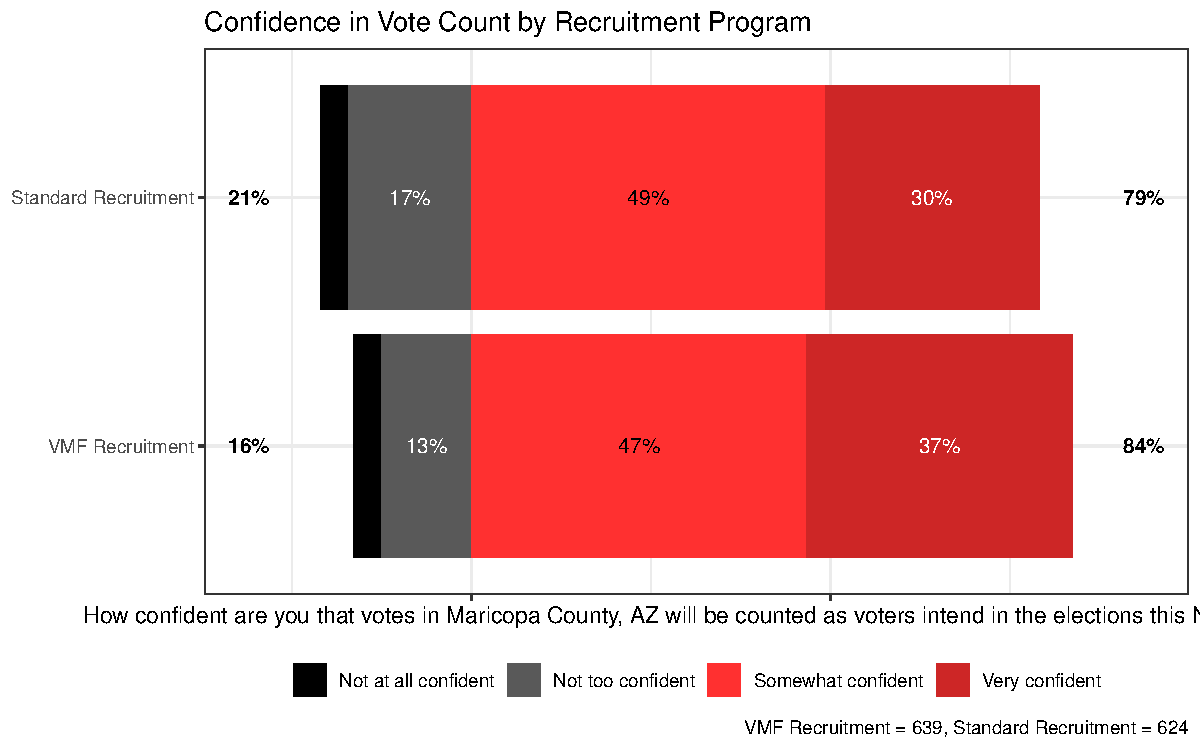
\includegraphics{index_files/figure-pdf/fig-q19-likert-1.pdf}

}

\end{figure}%

Importantly, the effects are generally even larger among those expected
to be the most skeptical. For example, \textbf{among those who said that
they thought Joe Biden's election to president was not legitimate,
exposure to information about veterans and military family members
increases confidence overall by 15 percentage points (from 60\% to 75\%,
p\textless0.025)}. The bulk of this increase is driven by a shift in the
rate at which respondents feel very confident, going from 9\% in the
control (community) condition to 19\% in the treatment (veterans)
condition. The following figures illustrate these results.

\begin{figure}

\caption{\label{fig-q19-legit}Confidence in Vote Count by Beliefs of
2020 Election Legitimacy and Recruitment Program}

\centering{

\centering{

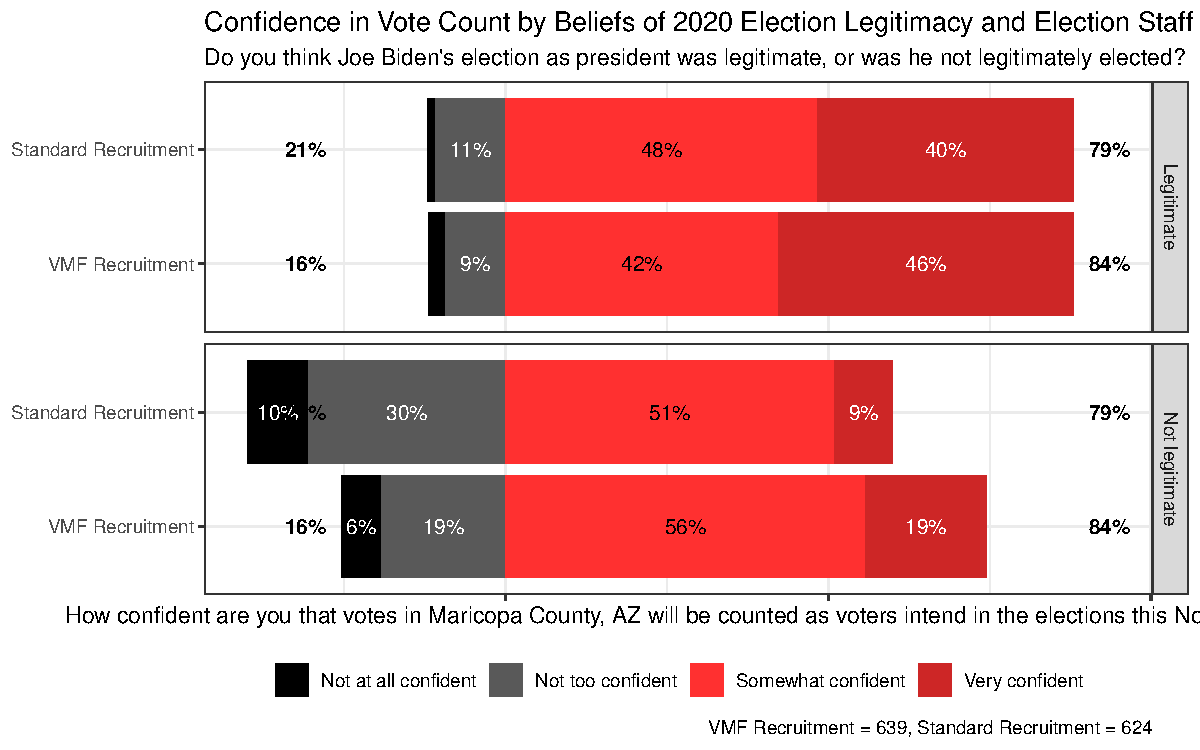
\includegraphics{index_files/figure-pdf/fig-q19-legit-1.pdf}

}

\subcaption{\label{fig-q19-legit}Proportion of confidence in vote count
by belief of Biden's election legitimacy and Experimental condition}

}

\end{figure}%

Veterans and military family members are also regarded highly by the
public for their commitment. \emph{Respondents were more likely to say
the elections workforce would be very committed to making sure the
elections held this November are fair and accurate when they heard that
veterans and military family members were being recruited to elections
jobs (by 9 percentage points, p\textless0.01)}.

\begin{figure}

\caption{\label{fig-q21-likert}Confidence in Commitment of Election
Staff and Volunteers by Recruitment Program}

\centering{

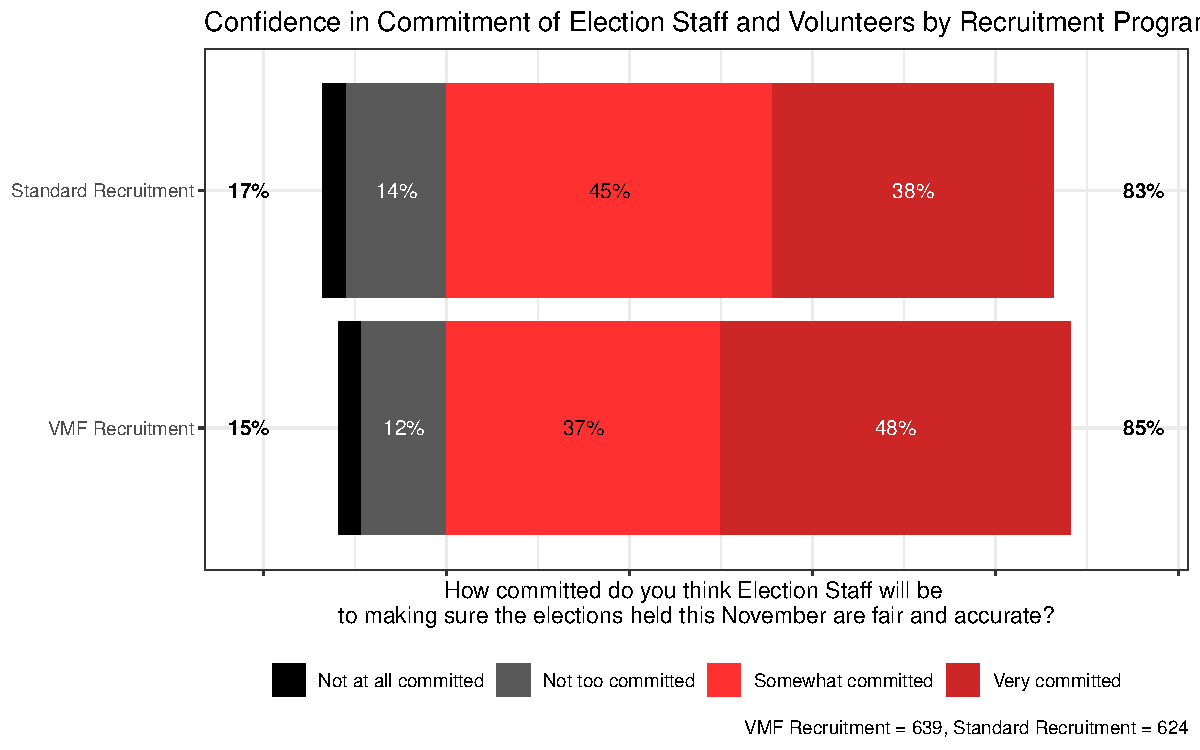
\includegraphics{index_files/figure-pdf/fig-q21-likert-1.pdf}

}

\end{figure}%

As shown in Figure~\ref{fig-q21-likert}, this increase is especially
noteworthy as it brings the percentage of those saying very committed to
nearly 50\% (from just under 38.5\% \% to 48\%).

\textbf{Information that election officials were recruiting veterans and
military family members also increased confidence that the voting
process in Maricopa County, AZ would be fair (by 7 percentage points,
p\textless0.01)}.

\begin{figure}

\caption{\label{fig-q22-likert}Confidence in Fair Voting Process by
Recruitment Program}

\centering{

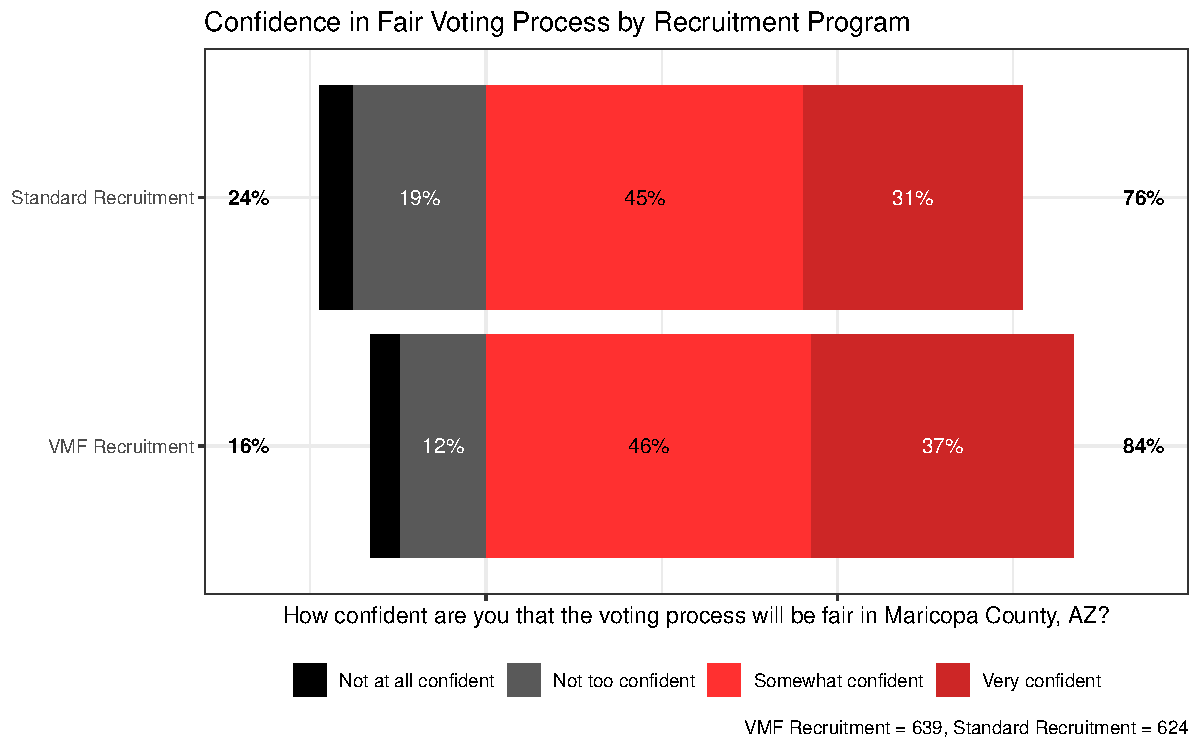
\includegraphics{index_files/figure-pdf/fig-q22-likert-1.pdf}

}

\end{figure}%

The bulk of this shift comes from an increase in the percentage of
people saying they were very confident (6 points, p\textless0.025).
\textbf{Again, the treatment effect was largest for those who said that
Joe Biden was not elected legitimately}. Whereas 57\% of those saying
Biden's victory was not legitimate were confident in the control
(community) condition, confidence rose 16 percentage points to 73\%
among those who believe Biden's election was not legitimate in the
treatment (veterans) condition.

\begin{figure}

\caption{\label{fig-q22-legit}Confidence in Fair Voting Process in
Maricopa County, AZ among those who believe Biden's 2020 election was
not legitimate}

\centering{

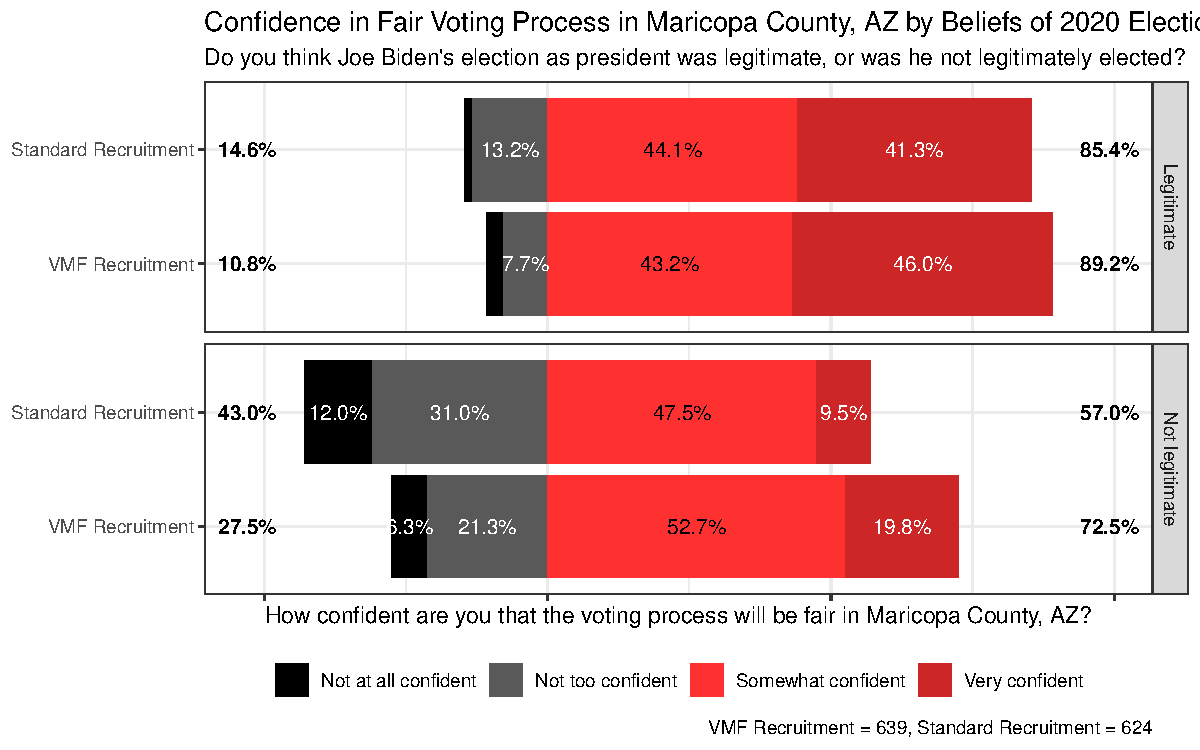
\includegraphics{index_files/figure-pdf/fig-q22-legit-1.pdf}

}

\end{figure}%

Although outcomes are subject to a wider variety of factors, the
veterans treatment also increased confidence that the outcomes would be
fair (by 4 percentage points, p\textless0.05), with a shift of 7
percentage points in the percentage saying they were very confident
(p\textless0.025).

\begin{figure}

\caption{\label{fig-q23-likert}Confidence in Fair Voting Outcomes by
Recruitment Program}

\centering{

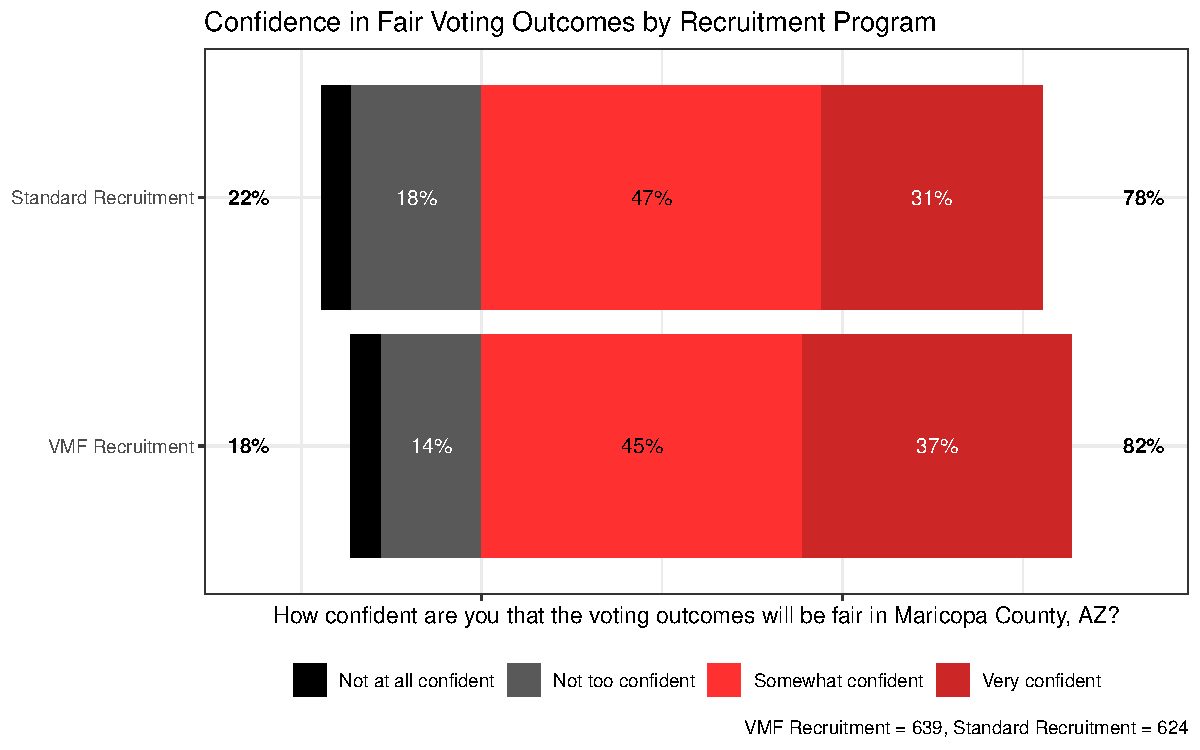
\includegraphics{index_files/figure-pdf/fig-q23-likert-1.pdf}

}

\end{figure}%

\subsubsection{Trust and Confidence in Election Security and Voter
Safety}\label{trust-and-confidence-in-election-security-and-voter-safety}

Attitudes relating to election security and safety were also improved as
a result of exposure to information that veterans and military family
members were being recruited to elections jobs. \textbf{The percentage
saying they were confident the election would be secure from hacking and
other technological threats was 7 points higher (p\textless0.01) in the
veterans condition}.

\begin{figure}

\caption{\label{fig-q24-likert}Trust in Election Systems Tech by
Recruitment Program}

\centering{

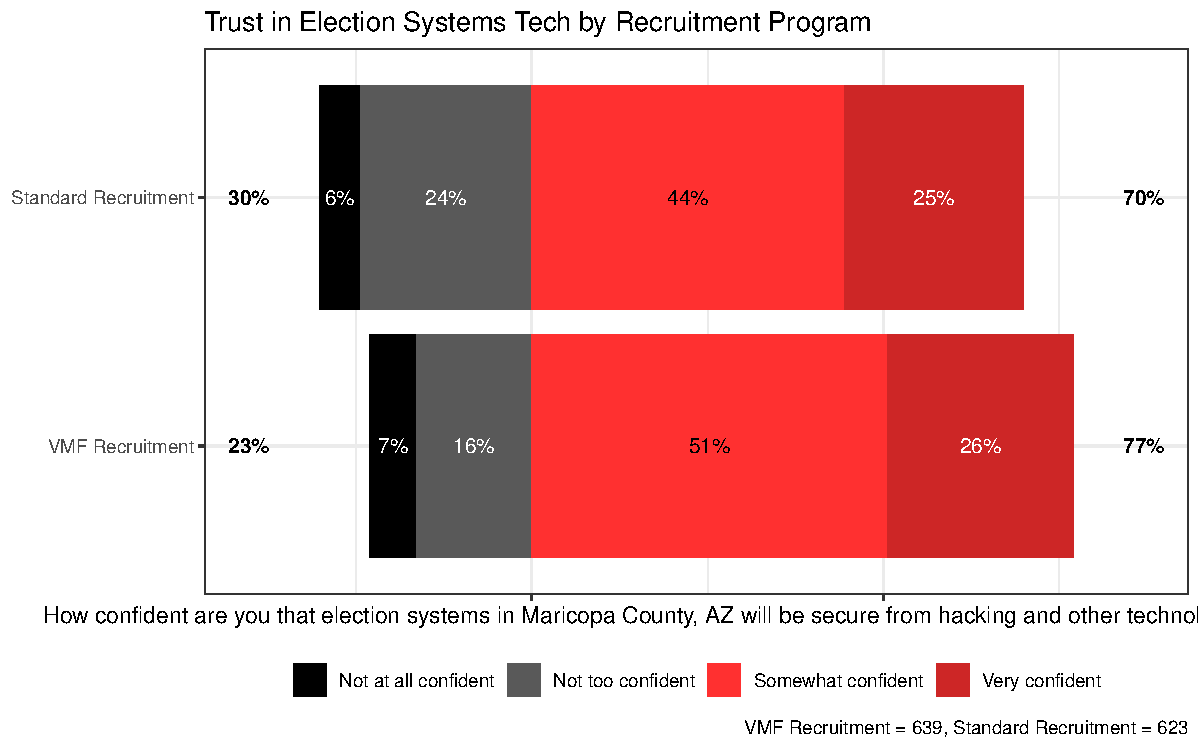
\includegraphics{index_files/figure-pdf/fig-q24-likert-1.pdf}

}

\end{figure}%

We assessed concerns for violence by asking how concerned voters in
Maricopa County, AZ should feel about potential violence, threats of
violence, or intimidation while voting in person at their local polling
place. The level of concern with potential violence, threats, and
intimidation was considerably lower (by 8 percentage points,
p\textless0.01) among those who read that veterans and military family
members were being recruited to the elections workforce. \textbf{In
other words, concerns over the prospect of violence, threats of
violence, and voter intimidation at election polling sites was far lower
among those who were given information that veterans and their family
members are being recruited to work as election staff compared to those
who were given information that made no mention of veterans and family
members.}

\begin{figure}

\caption{\label{fig-q25-likert}Concern for violence, threats, or voter
intimidation in Maricopa County, AZ by Recruitment Program}

\centering{

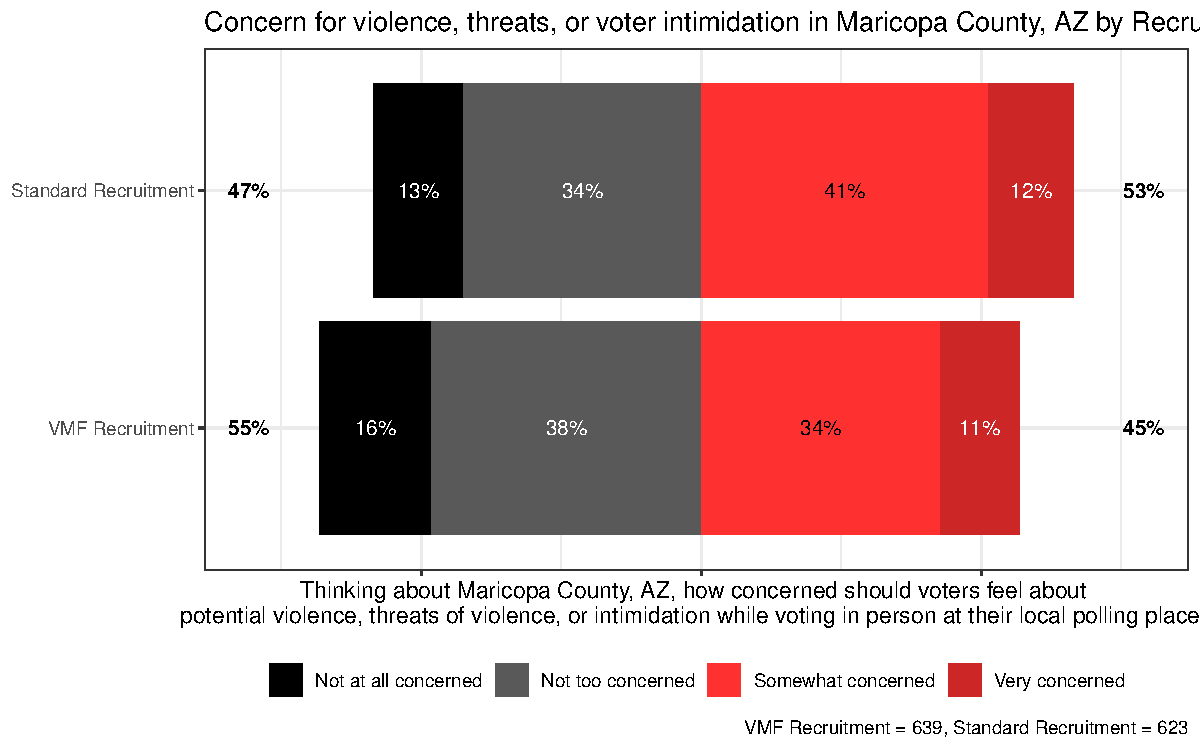
\includegraphics{index_files/figure-pdf/fig-q25-likert-1.pdf}

}

\end{figure}%

The size of this effect is especially significant because it brings the
level of concern (``Somewhat concerned'' and ``Very concerned'') below
the 50\% mark. That is, while a majority (53\%) of those who read about
a standard election staff recruitment program were at least somewhat
concerned, concerns for violence drop down to 45\% among those who
learned that officials of Maricopa County, AZ launched a program
designed specifically to recruit veterans and family members.
Additionally, those who learned about the VMF recruitment program were
more likely to say they were confident that polling places would be safe
places for voting in-person by 7 percentage points (p\textless0.01).

\begin{figure}

\caption{\label{fig-q26-likert}In-person voter safety in Maricopa
County, AZ by Recruitment Program}

\centering{

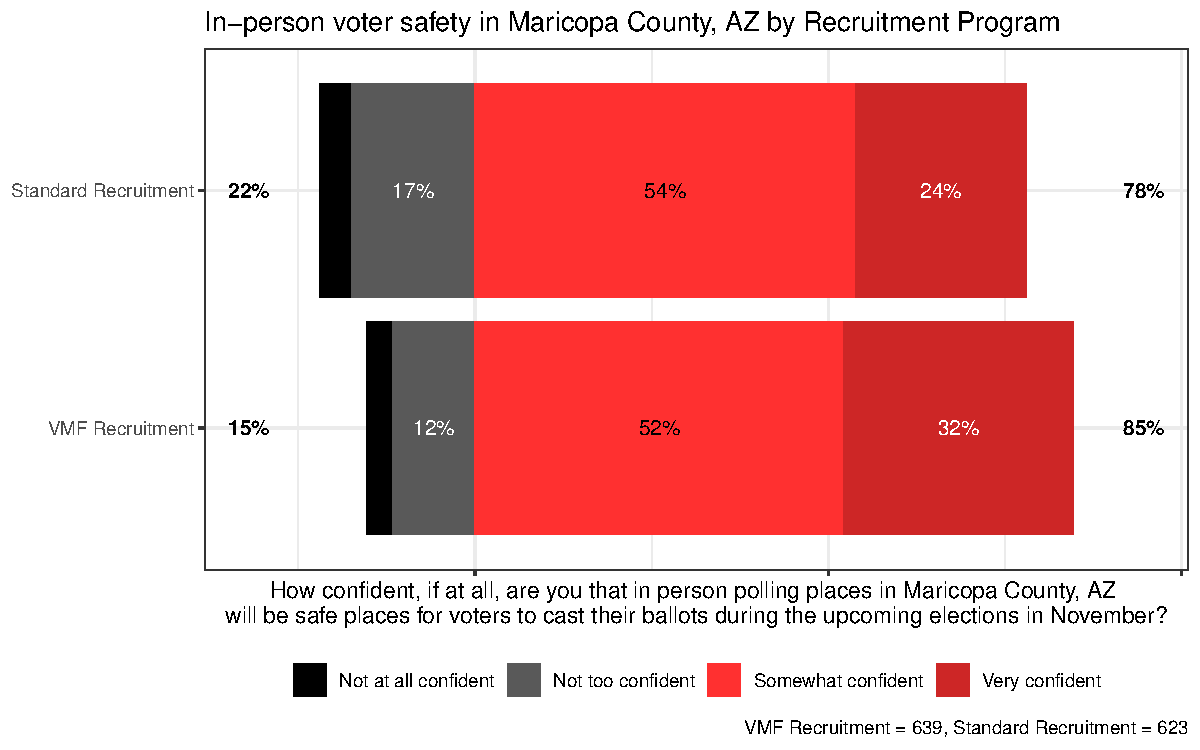
\includegraphics{index_files/figure-pdf/fig-q26-likert-1.pdf}

}

\end{figure}%

Note the nuanced distinction between the survey questions of
\textbf{?@fig-25-likert} and \textbf{?@fig-26-likert}: the former asks
how concerned \emph{the voters of Maricopa County, AZ should be} about
violence, etc., whereas the latter asks for the respondent's personal
judgement of \emph{how safe it will be in Maricopa County, AZ} to cast a
vote in-person. These two survey items use slightly different questions
to inquire about the same essential attitude---i.e., perceptions of
voter safety at the polls. While there were still a hefty proportion of
concern over the prospect of violence and voter safety at the polls
across the board, these results suggest that special efforts to recruit
veterans and their family members to work as election staff and
volunteers eases such concerns quite significantly.

Learning that Maricopa County, AZ was recruiting veterans and military
family members for elections jobs also led to improved performance
ratings for election officials there. In the veterans condition, those
saying they somewhat or strongly approve of the way election officials
are handling their jobs was 5 percentage points higher (p\textless0.05),
driven by a nearly 8 point increase in the percentage saying they
strongly approve of election officials (p\textless0.01).

\begin{figure}

\caption{\label{fig-q27-likert}Approval of Election Officials in
Maricopa County, AZ by Recruitment Program}

\centering{

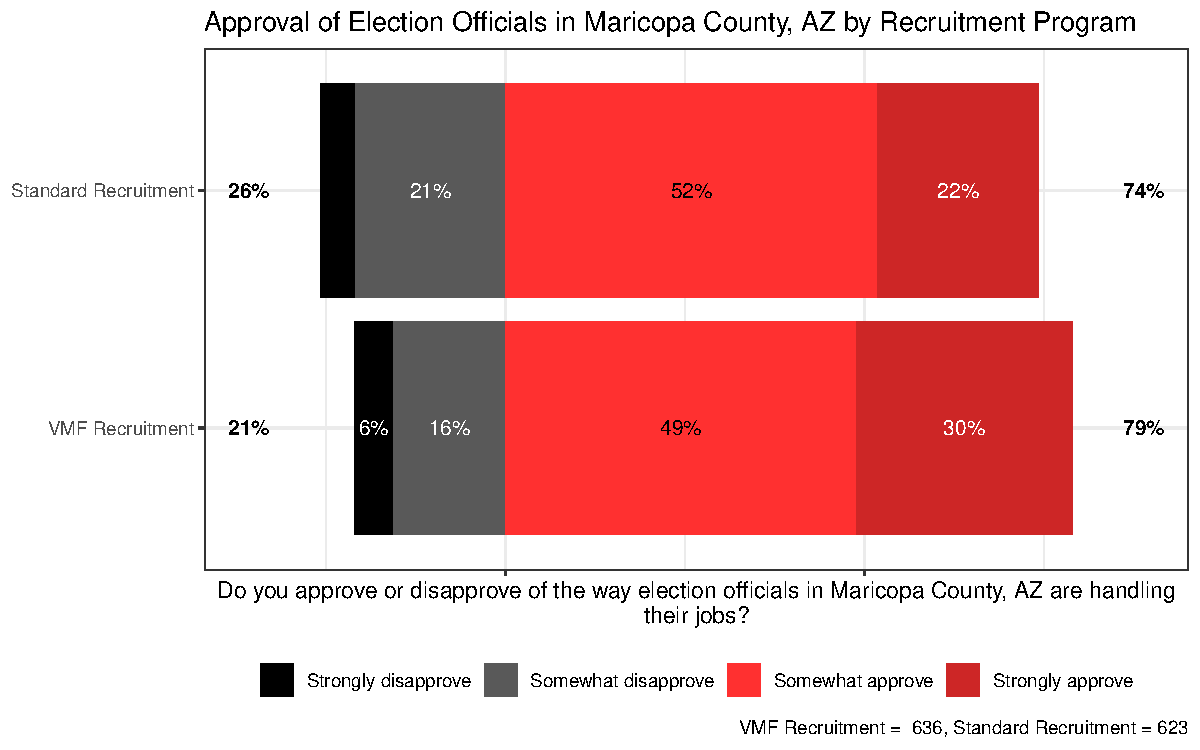
\includegraphics{index_files/figure-pdf/fig-q27-likert-1.pdf}

}

\end{figure}%

We also asked a general question about confidence that Maricopa County,
AZ elections officials would do a good job conduction elections this
November. Those who read about veterans and military family members were
more confident that election officials would do a good job conducting
the election than those who read about community members (by 4.5
percentage points, p \textless0.05).

\begin{figure}

\caption{\label{fig-20-likert}Confidence Election Officials in Maricopa
County, AZ will do a good job by Recruitment Program}

\centering{

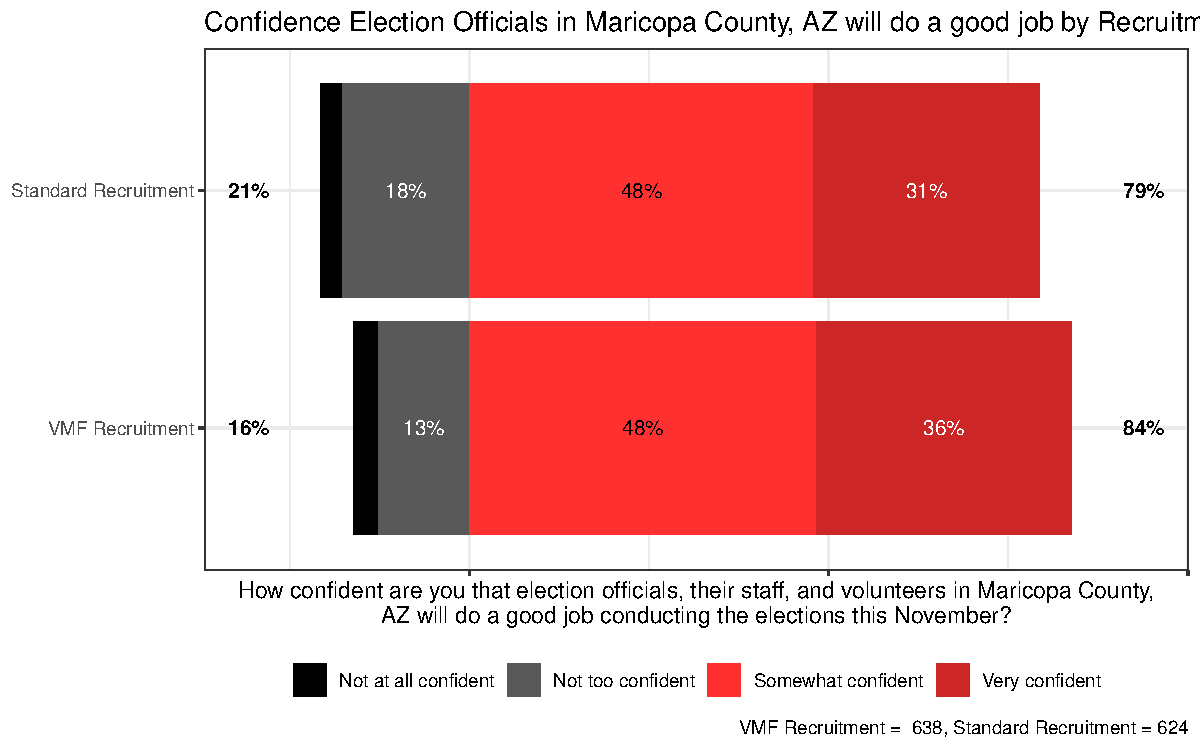
\includegraphics{index_files/figure-pdf/fig-20-likert-1.pdf}

}

\end{figure}%

Before asking a series of questions about election administration in
their own community, we asked how much respondents would like to see
their local community adopt a program for recruiting elections staff
similar to the one they read about in Maricopa County, AZ. Among those
in the community condition just under 73\% said their local area should
probably or definitely adopt the policy compared to over 77\% in the
veterans condition (difference of 5 percentage points, p\textless0.03).
The difference is driven entirely by an increase in enthusiasm (i.e.,
the likelihood of saying definitely should adopt is 5 points higher in
the veterans condition, p\textless0.025).

\begin{figure}

\caption{\label{fig-q29-likert}Approval of Election Officials in
Maricopa County, AZ by Recruitment Program}

\centering{

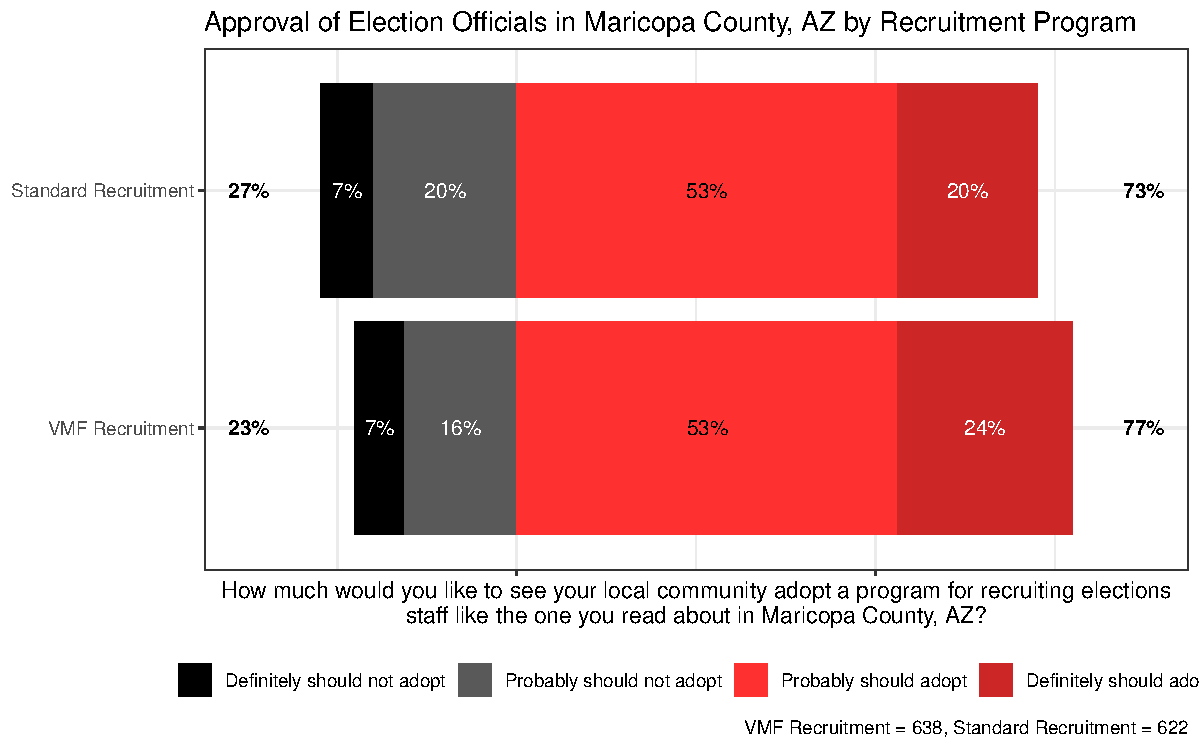
\includegraphics{index_files/figure-pdf/fig-q29-likert-1.pdf}

}

\end{figure}%

\newpage{}

\subsection{Expectation of Electoral
Fraud}\label{expectation-of-electoral-fraud}

Our survey also asked respondents a series of questions designed to
assess an individual's expectation of electoral fraud and voter
suppression in Maricopa County, AZ. Five statements were prefaced with
the question, ``How likely do you think any or all of the following will
happen during this year´s elections in Maricopa County, AZ?''. Survey
participants gave their expectations of the likelihood that each of the
following would occur in Maricopa County, Arizona this election cycle on
a scale of ``Not likely at all'', ``Not too likely'', ``Somewhat
likely'', and ``Very likely''.

\begin{enumerate}
\def\labelenumi{\arabic{enumi}.}
\tightlist
\item
  There will be voter fraud, that is, people who are not eligible to
  vote will vote, or vote more than once;
\item
  Many votes will not actually be counted
\item
  Many people will show up to vote and be told they are not eligible
\item
  A foreign country will tamper with the votes cast in this area to
  change the results
\item
  Election officials in Maricopa County, Arizona will try to discourage
  some people from voting
\end{enumerate}

\begin{figure}

\caption{\label{fig-q28-likert}Expectation of Electoral Fraud in
Maricopa County, AZ by Recruitment Program}

\centering{

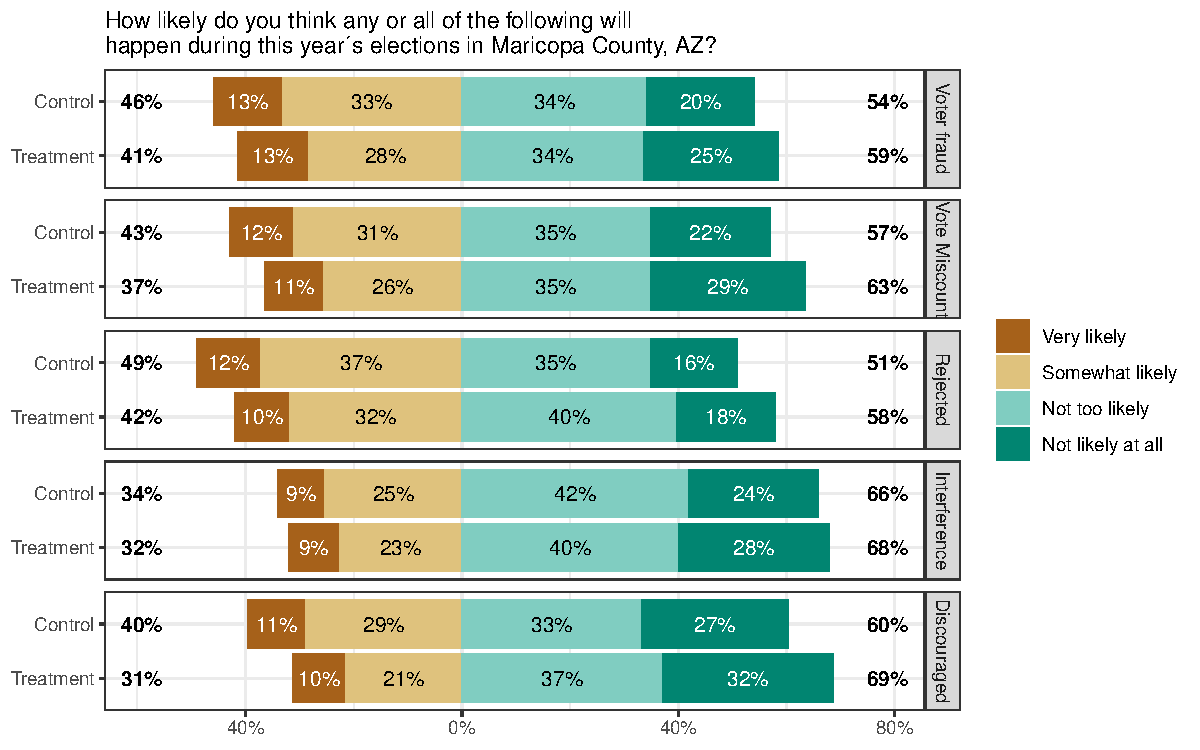
\includegraphics{index_files/figure-pdf/fig-q28-likert-1.pdf}

}

\end{figure}%

As Figure~\ref{fig-q28-likert} illustrates, \textbf{those in the
veterans condition were more likely to say that voter fraud was ``not
likely at all'' (by 5 percentage points, p\textless0.025). The
percentage saying that election officials will try to discourage people
from voting was not likely to occur in Maricopa County was 8 percentage
points higher among those who read that veterans and military family
members would be part of the elections workforce} (p\textless0.01, with
a shift of about 4 points among both those saying not too likely and not
likely at all). Additionally, in the veterans condition the percentage
saying that it was ``not likely at all'' that many votes will not
actually be counted was nearly 7 percentage points higher
(p\textless0.01), with a similar increase in the percentage saying it
was not likely (not too likely and not likely at all) that many people
will show up and be told they are not eligible (p\textless0.01).

When we asked about the likelihood that a foreign country would tamper
with votes in Maricopa County, AZ a larger percentage of those in the
veterans condition said this was ``not likely at all'' (by 4 percentage
points, p\textless0.07).

\newpage{}

\subsection{Impacts on Confidence}\label{impacts-on-confidence}

\begin{tcolorbox}[enhanced jigsaw, arc=.35mm, colbacktitle=quarto-callout-note-color!10!white, colframe=quarto-callout-note-color-frame, opacitybacktitle=0.6, left=2mm, titlerule=0mm, title=\textcolor{quarto-callout-note-color}{\faInfo}\hspace{0.5em}{Note}, coltitle=black, rightrule=.15mm, breakable, colback=white, toprule=.15mm, bottomtitle=1mm, toptitle=1mm, opacityback=0, leftrule=.75mm, bottomrule=.15mm]

Everything beyond this point is subject to change.

\end{tcolorbox}

We asked respondents to report how various features of election
administration would: 1) influence their confidence in the fairness and
accuracy of elections this November; and 2) influence their confidence
that voters would be safe from violence, threats of violence, or
intimidation while voting in-person this election. One of the primary
objectives was to determine whether recruiting veterans was preferable
to recruiting lawyers and college students, two other groups that are
commonly discussed as potential additions to the elections workforce.

\subsubsection{Impact on confidence in fairness and accuracy of
elections}\label{impact-on-confidence-in-fairness-and-accuracy-of-elections}

Survey participants responded to six statements, all prefaced with the
following,

\begin{quote}
``Regardless of whether any of these are actually the case, how would
the following impact your confidence in the fairness and accuracy of
elections conducted this November?''
\end{quote}

\begin{enumerate}
\def\labelenumi{\arabic{enumi}.}
\tightlist
\item
  Election officials test every machine used in the election to ensure
  they are secure.
\item
  Election officials conduct audits of ballots after every election to
  confirm the results were accurate.
\item
  Poll watchers affiliated with the political parties or candidates
  observe the election.
\item
  Election staff and volunteers include military veterans and their
  family members from the community\footnote{Two different versions of
    this statement was presented to survey participants. Half of the
    sample read the statement as, ``Election staff and volunteers
    \emph{include} military veterans and their family members from the
    community'', whereas the other half of the sample read, ``The
    \emph{majority} of election staff and volunteers consist of military
    veterans and their family members from the community.'' No
    significant differences in responses were observed between those who
    read one version of the statement over the other. However, the same
    was done for statements number 5 and 6 which concern ``lawyers from
    the community'' and ``college students from the community''.
    Significant differences were found when comparing responses between
    the different versions of these statements. See the appendix for
    further discussion on these results.}.
\item
  Election staff and volunteers include lawyers from the community.
\item
  Election staff and volunteers include college students from the
  community.
\end{enumerate}

For each statement, survey participants responded by selecting one of
five response options:

\begin{enumerate}
\def\labelenumi{\arabic{enumi}.}
\tightlist
\item
  Decrease confidence a lot
\item
  Decrease confidence somewhat
\item
  No impact on confidence
\item
  Increase confidence somewhat
\item
  Increase confidence a lot
\end{enumerate}

The primary interest concerned whether confidence in election fairness
would increase or decrease based on the composition of election staff
and volunteers. Of particular importance are responses to the statement
which asked respondents to consider whether inclusion of military
veterans and veteran's family members as election staff and volunteers
has any impact on their confidence in the fairness and accuracy of
elections in November.

\begin{figure*}

\centering{

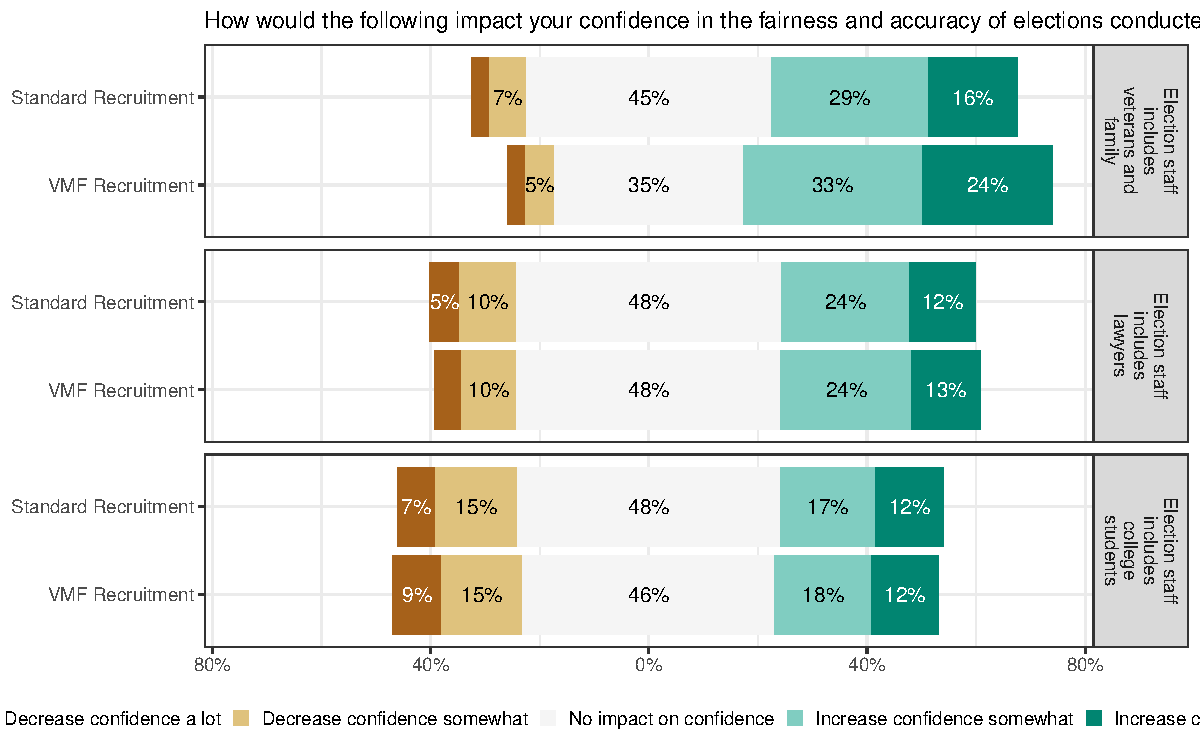
\includegraphics{index_files/figure-pdf/fig-q41-likert-1.pdf}

}

\caption{\label{fig-q41-likert}Impact on Confidence in Election Fairness
and Accuracy by Recruitment Program}

\end{figure*}%

Results displayed in Figure~\ref{fig-q41-likert} suggest that county
efforts to recruit veterans as election staff and volunteers does more
to increase one's confidence in the fairness and accuracy of elections
regardless of the experimental condition. That is, even for those who
were in the \emph{control} group, respondents reported that the
inclusion of veterans and their family members as election staff and
volunteers would increase confidence in the fairness and accuracy of
elections more than when election staff includes lawyers or college
students. This increase in confidence was 9\% percentage points higher
compared to when lawyers are included as election staff, and 16\%
percentage points higher than when election staff and volunteers are
said to include college students.

Moreover, Figure~\ref{fig-q41-likert} demonstrates a clear boost in
confidence when election staff includes veterans and family members,
especially for those who were in the treatment group. The percentage of
people who said their confidence in election fairness would increase
when election staff includes veterans was about 11.6\% percentage points
higher than those who said the same in the control group.

These results suggest that county efforts to recruit veterans as
election staff and volunteers does more to increase one's confidence in
the fairness and accuracy of elections, especially under the prospect
that election staff and volunteers would include veterans and their
family members.

These results suggest that reading a vignette about county efforts to
recruit veterans as election staff and volunteers does more to increase
one's confidence in the fairness and accuracy of elections, especially
under the prospect that election staff and volunteers would include
veterans and their family members.

\subsubsection{Impact on Confidence in Voter Safety at polling
sites}\label{impact-on-confidence-in-voter-safety-at-polling-sites}

The same analysis was conducted for questions that assessed the reported
impact on confidence that voters would be safe to vote in-person. Survey
participants provided responses to the same six statements as before,
which were all prefaced with the following question,

\begin{quote}
``How would the following impact your confidence that voters are safe
from violence, threats of violence, or intimidation while voting
in-person during elections this November?''
\end{quote}

Again, the bar graph below displays a clear boost among participants in
the treatment group who reported that their confidence in voter safety
would increase when election staff is said to include veterans and their
family members.

\begin{figure*}

\centering{

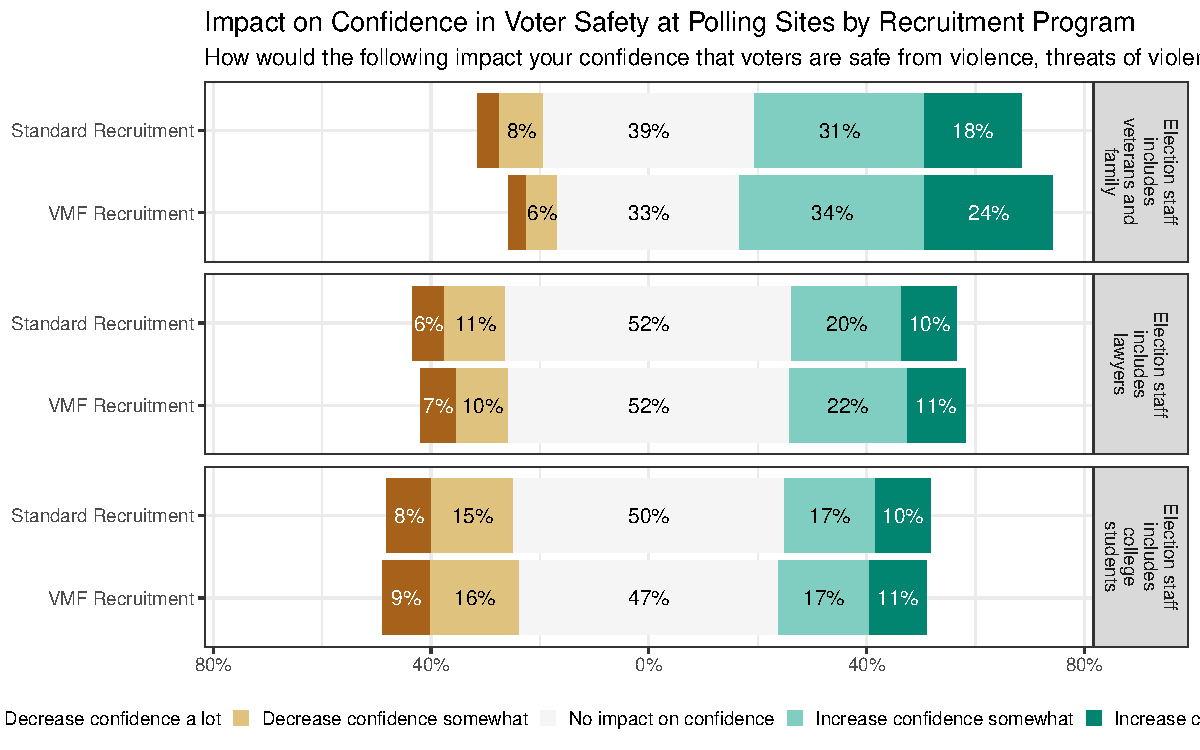
\includegraphics{index_files/figure-pdf/fig-q43-likert-1.pdf}

}

\caption{\label{fig-q43-likert}}

\end{figure*}%

The proportion of people who said their confidence in voter safety would
increase when election staff includes veterans was about 8.4 percentage
points higher than those who said the same in the control group.

\section{Sample Demographics and
Balance}\label{sample-demographics-and-balance}

The decision was made to exclude any respondents who didn't complete the
survey. There were a total of 125 respondents who started but didn't
finish the survey. Of those 125, 105 quit before reaching
\texttt{Q40\_1}, whereas the rest exited the survey after that
question\footnote{Due to the programming of the survey, respondents were
  randomly assigned to either question set `A' or question set `B'. The
  grouping variable in the data set is \texttt{Qset}. Those respondents
  assigned to \texttt{Qset\ A} answered questions \texttt{Q41} and
  \texttt{Q43}; those assigned to \texttt{Qset\ B} answered question
  \texttt{Q44} and \texttt{Q46}. For each question, respondents were
  presented six statements and selected a response on a 5-point scale
  from ``Decrease Confidence a lot'' to ``Increase confidence a lot''.
  The six statements were the same for each question. This resulted in
  six variables per question within the data set (e.g., Q41\_1 to
  Q41\_6), where each variable consisted of responses to one of the six
  particular statements. Tests of differences in proportion between the
  question sets determined that responses were mostly equivalent between
  question sets (i.e., no statistically significant differences between
  proportions) except for the fifth and sixth statements pertaining to
  lawyers and college students. More detailed information on the results
  of this analysis are given in a supplementary document.}.

\texttt{NA} missing values from the \texttt{Qset} variable removes those
105 partial survey responses, i.e., respondents who quit prior to
reaching \texttt{Q40}.

\begin{table}

\caption{\label{tbl-demog}Survey sample characteristics by treatment
condition}

\centering{

\begingroup\fontsize{13}{15}\selectfont

\begin{tabu} to \linewidth {>{\raggedright}X>{\raggedright}X>{\raggedright}X>{\raggedright}X}
\toprule
  & Standard Recruitment & VMF Recruitment & Overall\\
\midrule
 & (N=624) & (N=639) & (N=1263)\\
\addlinespace[0.3em]
\multicolumn{4}{l}{\textbf{Age categorized into eight groups}}\\
\hspace{1em}18-24 & 56 (9.0\%) & 51 (8.0\%) & 107 (8.5\%)\\
\hspace{1em}25-34 & 107 (17.1\%) & 127 (19.9\%) & 234 (18.5\%)\\
\hspace{1em}35-44 & 130 (20.8\%) & 121 (18.9\%) & 251 (19.9\%)\\
\hspace{1em}45-54 & 113 (18.1\%) & 110 (17.2\%) & 223 (17.7\%)\\
\hspace{1em}55-64 & 124 (19.9\%) & 115 (18.0\%) & 239 (18.9\%)\\
\hspace{1em}65-74 & 70 (11.2\%) & 74 (11.6\%) & 144 (11.4\%)\\
\hspace{1em}75-84 & 20 (3.2\%) & 36 (5.6\%) & 56 (4.4\%)\\
\hspace{1em}85-92 & 4 (0.6\%) & 5 (0.8\%) & 9 (0.7\%)\\
\addlinespace[0.3em]
\multicolumn{4}{l}{\textbf{What is your current gender?}}\\
\hspace{1em}Male & 285 (45.7\%) & 307 (48.0\%) & 592 (46.9\%)\\
\hspace{1em}Female & 329 (52.7\%) & 326 (51.0\%) & 655 (51.9\%)\\
\hspace{1em}Other/Refused & 10 (1.6\%) & 6 (0.9\%) & 16 (1.3\%)\\
\addlinespace[0.3em]
\multicolumn{4}{l}{\textbf{Primary race reported by respondent}}\\
\hspace{1em}White or Caucasian & 476 (76.3\%) & 493 (77.2\%) & 969 (76.7\%)\\
\hspace{1em}Black or African American & 82 (13.1\%) & 79 (12.4\%) & 161 (12.7\%)\\
\hspace{1em}American Indian & 10 (1.6\%) & 12 (1.9\%) & 22 (1.7\%)\\
\hspace{1em}Asian & 26 (4.2\%) & 30 (4.7\%) & 56 (4.4\%)\\
\hspace{1em}Other & 30 (4.8\%) & 25 (3.9\%) & 55 (4.4\%)\\
\addlinespace[0.3em]
\multicolumn{4}{l}{\textbf{Highest level of education completed}}\\
\hspace{1em}Less than high school degree & 20 (3.2\%) & 14 (2.2\%) & 34 (2.7\%)\\
\hspace{1em}High school graduate (high school diploma or equivalent including GED) & 152 (24.4\%) & 174 (27.2\%) & 326 (25.8\%)\\
\hspace{1em}Some college but no degree & 141 (22.6\%) & 140 (21.9\%) & 281 (22.2\%)\\
\hspace{1em}Associate degree in college (2-year) & 69 (11.1\%) & 68 (10.6\%) & 137 (10.8\%)\\
\hspace{1em}Bachelor's degree in college (4-year) & 166 (26.6\%) & 156 (24.4\%) & 322 (25.5\%)\\
\hspace{1em}Master's degree & 61 (9.8\%) & 69 (10.8\%) & 130 (10.3\%)\\
\hspace{1em}Doctoral degree & 5 (0.8\%) & 13 (2.0\%) & 18 (1.4\%)\\
\hspace{1em}Professional degree (JD, MD) & 10 (1.6\%) & 5 (0.8\%) & 15 (1.2\%)\\
\addlinespace[0.3em]
\multicolumn{4}{l}{\textbf{Party ID 3 categories, with true Independents}}\\
\hspace{1em}Republican & 261 (41.8\%) & 276 (43.2\%) & 537 (42.5\%)\\
\hspace{1em}Democrat & 282 (45.2\%) & 283 (44.3\%) & 565 (44.7\%)\\
\hspace{1em}Independent & 81 (13.0\%) & 79 (12.4\%) & 160 (12.7\%)\\
\hspace{1em}Missing & 0 (0\%) & 1 (0.2\%) & 1 (0.1\%)\\
\addlinespace[0.3em]
\multicolumn{4}{l}{\textbf{Have you ever served in the Armed Forces?}}\\
\hspace{1em}Yes & 53 (8.5\%) & 68 (10.6\%) & 121 (9.6\%)\\
\hspace{1em}No & 571 (91.5\%) & 571 (89.4\%) & 1142 (90.4\%)\\
\addlinespace[0.3em]
\multicolumn{4}{l}{\textbf{Are you now serving in the Armed Forces?}}\\
\hspace{1em}Yes & 5 (0.8\%) & 10 (1.6\%) & 15 (1.2\%)\\
\hspace{1em}No & 48 (7.7\%) & 58 (9.1\%) & 106 (8.4\%)\\
\hspace{1em}Missing & 571 (91.5\%) & 571 (89.4\%) & 1142 (90.4\%)\\
\addlinespace[0.3em]
\multicolumn{4}{l}{\textbf{Member of immediate family served or is currently serving}}\\
\hspace{1em}Yes & 215 (34.5\%) & 223 (34.9\%) & 438 (34.7\%)\\
\hspace{1em}No & 409 (65.5\%) & 416 (65.1\%) & 825 (65.3\%)\\
\addlinespace[0.3em]
\multicolumn{4}{l}{\textbf{Turnout 2020}}\\
\hspace{1em}Didn't vote & 129 (20.7\%) & 117 (18.3\%) & 246 (19.5\%)\\
\hspace{1em}Unsure/Ineligible & 49 (7.9\%) & 52 (8.1\%) & 101 (8.0\%)\\
\hspace{1em}Voted & 446 (71.5\%) & 470 (73.6\%) & 916 (72.5\%)\\
\addlinespace[0.3em]
\multicolumn{4}{l}{\textbf{Who did you vote for?}}\\
\hspace{1em}Donald Trump & 214 (34.3\%) & 222 (34.7\%) & 436 (34.5\%)\\
\hspace{1em}Joe Biden & 252 (40.4\%) & 272 (42.6\%) & 524 (41.5\%)\\
\hspace{1em}Other & 30 (4.8\%) & 28 (4.4\%) & 58 (4.6\%)\\
\hspace{1em}Missing & 128 (20.5\%) & 117 (18.3\%) & 245 (19.4\%)\\
\addlinespace[0.3em]
\multicolumn{4}{l}{\textbf{Do you plan to vote?}}\\
\hspace{1em}Yes & 500 (80.1\%) & 532 (83.3\%) & 1032 (81.7\%)\\
\hspace{1em}No & 56 (9.0\%) & 54 (8.5\%) & 110 (8.7\%)\\
\hspace{1em}Undecided & 68 (10.9\%) & 53 (8.3\%) & 121 (9.6\%)\\
\bottomrule
\multicolumn{4}{l}{\rule{0pt}{1em}Table reflects column percentages.}\\
\end{tabu}
\endgroup{}

}

\end{table}%

\section{Appendix: Survey Experiment
Vignettes}\label{appendix-survey-experiment-vignettes}

\begin{figure}

\begin{minipage}{0.50\linewidth}

\centering{

\subsubsection{Treatment Vignette}\label{treatment-vignette}

\textbf{Local Military Veterans Recruited for Election Jobs in Maricopa
County}\\
\strut \\
\strut ~~PHOENIX (AP) --- Election officials in Maricopa County,
Arizona, announced a program designed to recruit military veterans and
their family members from the community to serve as election
administrators, including election polling place workers, temporary
workers, and full-time staff. As the U.S. general elections in November
near, election officials must fill several thousand temporary positions
and hundreds of other open positions to ensure sufficient staffing for
the 2024 elections and beyond.\\
\strut \\
\strut ~~Army veteran Jordan Braxton just joined the elections
workforce. Jordan believes their role is important to ensuring a secure,
accurate, and transparent election, ``Many places are short on staff
this election cycle. I served my country in the Army, and I want to do
my part as a veteran and a citizen to ensure that everyone trusts the
process and the outcome of the election.''

}

\subcaption{\label{fig-treatment}Text of the Treatment Condition:
Recruitment of Veterans and Military Family Members}

\end{minipage}%
%
\begin{minipage}{0.50\linewidth}

\centering{

\subsubsection{Control Vignette}\label{control-vignette}

\textbf{Local Residents Recruited for Election Jobs in Maricopa
County}\\
\strut \\
\strut ~~PHOENIX (AP) ---Election officials in Maricopa County, Arizona,
announced a program to recruit members of the community to serve as
election administrators, including election polling place workers,
temporary workers, and full-time staff. As the U.S. general elections in
November near, election officials must fill several thousand temporary
positions and hundreds of other open positions to ensure sufficient
staffing for the 2024 elections and beyond.\\
\strut \\
\strut ~~Jordan Braxton just joined the elections workforce. Jordan
believes their role is important to ensuring a secure, accurate, and
transparent election, ``Many places are short on staff this election
cycle. I want to do my part as a citizen to ensure that everyone trusts
the process and the outcome of the election.''

}

\subcaption{\label{fig-control}Text of the Control Condition:
Recruitment of Community Members}

\end{minipage}%

\caption{\label{fig-vignettes}Fabricated Article Vignettes utilized as
Experimental Stimulus}

\end{figure}%




\end{document}
